\section{Approach to Discover the Control-Flow Perspective}
\label{sec:approach}

% In this section we illustrate the steps of the our technique for gathering insights on the software project (i.e., \gls{pobp}). Further, we discuss the design principles implemented by our prototype. 

% \subsection{Application scenario}

% Let us exemplify how our technique should help the project manager through the following four-step scenario.  
% First, using a \gls{gui}, a project manager should be able to analyze the project (i.e., explicitly see what activities are being done and when). She might observe a spike in a specific activity, for instance development. She notices that this is an unusual observation and she reports it for further investigation. This behaviour involves an exploration of the domain data in order to find interesting patterns. 
% Second, the manager describes this spike by using the information about the activity in which it occurred (e.g., in development and in testing), the time period (i.e., day, week, or month), the files and the resources involved. This description is needed in order to make the observation explicit and define it for further analysis.  
% Third, the manager crosses different observations on the data. She finds out that in the day before there were no changes by the resources in charge of that specific activity. She also observes that other resources who should not work on files affected by the spike, have actually made changes to those files. After cross-checking the resource occupancy with the day before, she finds out that actually resources were assigned bigger tasks which were not possible to be solved in the same day. That is why there was relatively little amount of work in the previous day and a sudden spike in the following day. 
% Fourth, the project manager notices more spikes in the process at different points in time. She hypothesizes that work distribution is not fair. She consults the KPIs and finds out that indeed the work inequality index is high. This confirms her hypothesis and explains why other resources also have made changes to files they were not in charge of. Finally, all these clues enable the organization to improve their development process.

% \subsection{Overview of the technique}


We developed a technique that addresses the identified requirements according to the process model in \Cref{fig:approach-overview}. 
This process starts when an event log from \gls{vcs} needs to be analyzed, ends with a final visualization of project insights, and consists of four steps.
First, an event log from \gls{vcs} is taken as an input. In this step, an \gls{etl} procedure is followed to obtain a structured event log which is easily processed in the next steps. Second, the activities are discovered based on file changes. Third, project related \glspl{kpi} are computed. Fourth, a visualization that summarizes the results of the previous two steps is provided to the project manager. In the following, we provide the implementation details of this process.

\begin{figure}[]
    \centering
    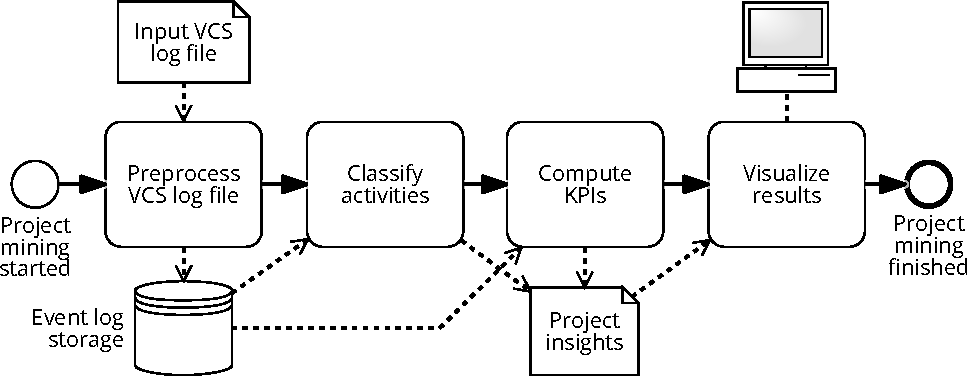
\includegraphics[width=.9\textwidth]{Project-mining-2-Mining-Type-of-Work/figures/overview}
    \caption{Overview of the approach}
    \label{fig:approach-overview}
\end{figure}


% \subsection{Implementation}

% This section presents the implementation of our technique to extract the type of work and several KPIs from a \gls{vcs} log.

\subsection{Preprocess VCS log file}

The input of this phase is a log in the unified diff format, which is supported
by the major \glspl{vcs}, such as Git and Subversion. The information retrieved by the \gls{vcs} is configurable by the user. More specifically, it is possible to obtain the basic information shown in \Cref{lst:git-log} along with details on the differences among versions of the same file (i.e., which and how many lines changed from version 1 to version 2 of file X). In order to extract such information, the raw event log is parsed. We used the parser from  \citep{DBLP:conf/bpm/BalaRGBMS17}. This parser generates events which are then stored into a \gls{dbms} for further processing. 

\Cref{fig:er-diagram} provides the \gls{er} model to represent the entities and relationships that are needed to capture an event. The entity \textsl{Project} models the software project at hand. By including this entity in the data model, we can gather data over multiple projects and store them in the same data store. \textsl{User} is the user who performs change operations on the files. \textsl{Commit} represents the status of the repository at a given point in time. Commits must contain a revision number, a timestamp and the user who issued them. \textsl{File} is a single file of the repository identified by its full path. \textsl{Edit} captures the change as numbers of lines added to or removed from a file. This step fulfills \textbf{R1}.

\begin{figure}[]
    \centering
    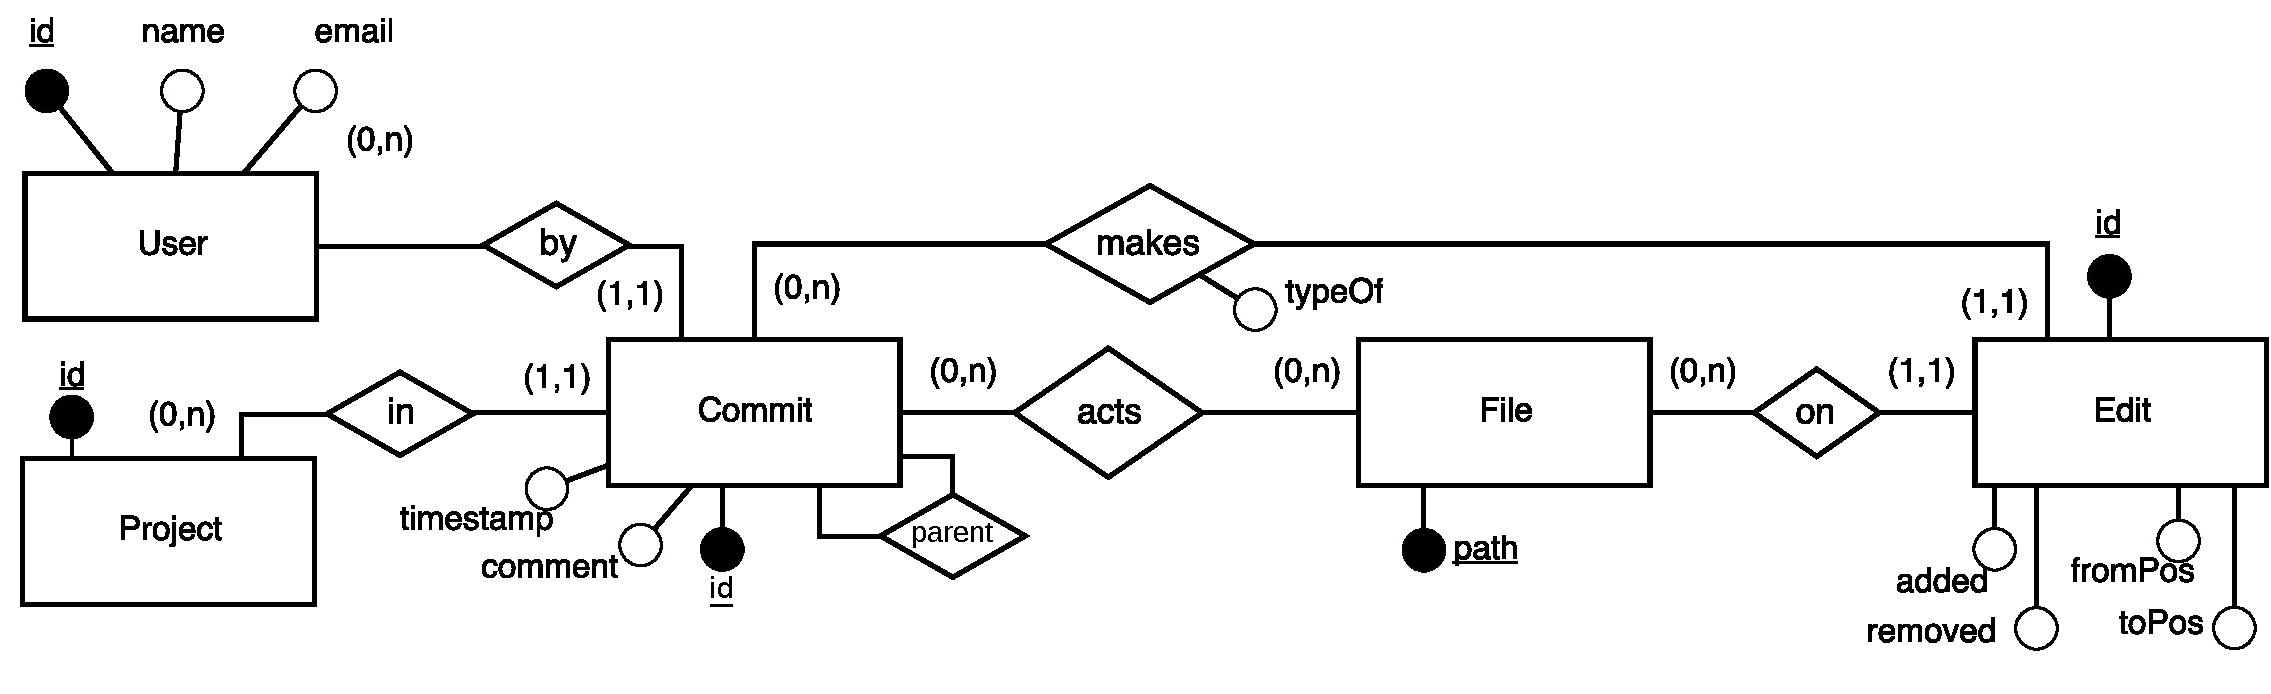
\includegraphics[width=\textwidth]{figures/CommitLogER}
    \caption{ER diagram capturing the entities and relationships of a software repository}
    \label{fig:er-diagram}
\end{figure}


\subsection{Classify activities}


Having the data stored in a \gls{dbms}, enables us to run several analyzes already at this level by simply issuing SQL queries. For example, we can obtain all changes that happened to single files during their lifetime. For the scope of this work, we collect all the file paths, all the changes that happened to files, the amount of change in terms of \gls{loc}, the type of change (e.g., addition, modification, deletion), the commit identifier, and the user who did the change. 
Next, we automatically categorize the type of change. For this, we apply regular expression on path attribute using the classes provided by literature \citep{DBLP:journals/ese/VasilescuSGM14}. 
Examples of classes are  \textsl{Documentation}, \textsl{Image}, \textsl{Testing}, \textsl{Coding}, \textsl{User interface}, etc. There are in total fourteen classes. When a type of change does not belong to any class, it is put under the category \textsl{Unknown}.

% Please add the following required packages to your document preamble:
% \usepackage{booktabs}
% \usepackage{graphicx}
\begin{table}[!htbp]
\centering
\caption{Set of activities that are discovered and main regular expressions}
\label{tab:regex}
\resizebox{\textwidth}{!}{%
% \scriptsize
\begin{tabular}{@{}p{2.2cm}p{2.1cm}p{7cm}@{}}
\toprule
\multicolumn{1}{c}{\textbf{Activity}} &
  \multicolumn{1}{c}{\textbf{Abbreviation}} &
  \multicolumn{1}{c}{\textbf{Regular Expression}} \\ \midrule
  Unknown &
  unknown &
  .* \\
Documentation &
  doc &
  .*\textbackslash{}/doc(-?)book(s?)\textbackslash{}/.* .*\textbackslash{}/info .*\textbackslash{}.txt((\textbackslash{}.bak)?) .*\textbackslash{}.man .*\textbackslash{}.tex \\
Image &
  img &
  .*\textbackslash{}.jpeg .*\textbackslash{}.bmp .*\textbackslash{}.chm .*\textbackslash{}.vdx .*\textbackslash{}.gif \\
Localization &
  loc &
  .*\textbackslash{}/locale(s?)\textbackslash{}/.* .*\textbackslash{}.po($\sim$?) .*\textbackslash{}.charset($\sim$?) \\
User interface &
  ui &
  .*\textbackslash{}.ui .*\textbackslash{}.gladep(\textbackslash{}\textbackslash{}d?)((\textbackslash{}.bak)?)($\sim$?) .*\textbackslash{}.theme \\
Multimedia &
  media &
  .*\textbackslash{}.mp3 .*\textbackslash{}.mp4 .*\textbackslash{}/media(s?)\textbackslash{}/.* .*\textbackslash{}.ogg \\
Code &
  code &
  .*\textbackslash{}.jar($\sim$?) .*\textbackslash{}/src\textbackslash{}/.* .*\textbackslash{}.r((\textbackslash{}.swp)?)($\sim$?)) .*\textbackslash{}.py((\textbackslash{}.swp)?)($\sim$?) .*\textbackslash{}.php((\textbackslash{}.swp)?)(\textbackslash{}\textbackslash{}d?)($\sim$?) \\
Meta &
  meta &
  .*\textbackslash{}.svn(.*) .*\textbackslash{}.git(.*) .*\textbackslash{}.cvs(.*) \\
Configuration &
  config &
  .*\textbackslash{}.conf .*\textbackslash{}.cfg .*\textbackslash{}.project .*\textbackslash{}.ini .*\textbackslash{}.prefs \\
Build &
  build &
  .*\textbackslash{}.cmake .*\textbackslash{}/install-sh .*\textbackslash{}/build\textbackslash{}/.* .*makefile.* \\
Development documentation &
  devdoc &
  .*readme.* .*\textbackslash{}/changelog.* .*\textbackslash{}/devel(-?)doc(s?)\textbackslash{}/.* \\
Database &
  db &
  .*\textbackslash{}.sql .*\textbackslash{}.sqlite .*\textbackslash{}.mdb .*\textbackslash{}.db \\
Test &
  test &
  .*\textbackslash{}.test(s?)\textbackslash{}/.* .*\textbackslash{}/.*test\textbackslash{}..* .*/test.*\textbackslash{}..* \\
Library &
  lib &
  .*\textbackslash{}/library\textbackslash{}/.* .*\textbackslash{}/libraries\textbackslash{}/.* \\ \bottomrule
\end{tabular}%
 }
\end{table}

We have adapted the regular expressions to our case and enriched the list of rules from literature. \Cref{tab:regex} shows the activity types and the main regular expressions we use to classify files onto specific types of work. For the sake of space, the majority of the regular expressions is left out. The reader can access the full list of regular expressions on our GitHub repository whose link is provided in the following section.

\lstset{
  basicstyle={\normalsize\ttfamily}}

For the categorization we consider both the extension of the file and its path. For example, a file with the path \lstinline{/test/file.java} is labelled as \textsl{Testing} rather than \textsl{Coding}. To achieve this, we sort the matching rules in order of specificity. 
At a higher level, a commit involves multiple files. In order to fit the commit into a specific class, we rely on majority voting as follows. We iterate over the list of changes affected by the commit and sort the number of changes by their activity and the amount of change. We select the activity that is associated to the highest number of changes. With this step we fulfill \textbf{R2}.

\subsection{Compute KPIs}

According to the process already presented in \Cref{fig:approach-overview}, we compute \glspl{kpi} with the help of the \gls{dbms}. This allows for a customized set of \glspl{kpi} to be implemented. In the scope of this paper, we reproduced some of the main \glspl{kpi} form literature \citep{DBLP:journals/ese/VasilescuSGM14}. We divide them into basic (absolute and relative) and specialization metrics. Basic metrics focus on descriptive statistics such as frequency counts of how many times each user works on a file. Specialization metrics focus on the measuring imbalance of work towards a specific file or author. Imbalance is captured by the Gini inequality index \citep{gini1921measurement}.
We implemented the following basic project metrics: \gls{pw}, \gls{tw}, \gls{nap}, \gls{ntp}. Furthermore, we also implemented the following specialization metrics: \gls{pis}, \gls{rpis}, and \gls{rpws}. 

Let $U$ be the set of all unique users in the project, $T$ the set of all activities in the project. Files that were edited in the context of a commit can be associated to a user $u \in U$ and an activity $t \in T$ computed as described above. 
We adapted the definition of \glspl{kpi} from literature to support the extraction of information about the activity types as follows. As a first step, we redefine the two basic \glspl{kpi} that are involved in the calculation of all other \glspl{kpi}. 
%\begin{definition}[UTW]
\gls{utw} is the number of files relative to activity $t$, a user $u$ edits over the entire history of the activity.
%\end{definition}
%\begin{definition}[UTI]
\gls{uti} is 1 if a user $u$ has been involved in (i.e., has edited at least once) a file with activity $w$. It is 0 otherwise. 
%\end{definition}
Finally, using these definitions, we can present in \Cref{tab:kpis-computation} how the rest of the \glspl{kpi} is computed. With this step we fulfill \textbf{R3}.\\\hfill

% Please add the following required packages to your document preamble:
% \usepackage{booktabs}
% \usepackage{graphicx}
\begin{table}[]
\setlength\belowcaptionskip{-20pt}
\centering
% \scriptsize
\caption{\glspl{kpi} computation details}
\label{tab:kpis-computation}
% \resizebox{\textwidth}{!}{%
\begin{tabular}{@{}m{1.5cm}m{6cm}m{4cm}@{}}
\toprule
\textbf{KPI} & \textbf{Description}                           & \textbf{Calculation}                     \\ \midrule
\gls{pw}     & (absolute) project workload                    & $\sum_{t \in T, u \in U} \gls{utw}(t,u)$ \\
\gls{tw} (t) & workload of a specific activity  & $\sum_{u \in U} \gls{utw}(t,u) $         \\
\gls{nap}    & number of authors in the project               & $\sum_{u_j \in U} j$                     \\
\gls{ntp}    & number of activities in the project         & $\sum_{t_j \in T} j$                     \\
\gls{pis}  & specialization of user involvement the activities of the project               & $Gini_{{t_k} \in T} (\sum_{u \in U}\gls{uti}(u, t_k))$                \\
\gls{rpis} & specialization of relative user involvement over the activities of the project & $Gini_{{t_k} \in T} ( \frac{\sum_{u \in U} \gls{uti}(u, t_k)}{ \gls{nap}} ) $ \\
\gls{rpws} & specialization of relative workload across all activities in the project       & $Gini_{{t_k} \in T} ( \frac {\sum_{u \in U} \gls{utw}(u, t_k) } { \gls{tw}})$  \\ \bottomrule
\end{tabular}%
% }
\end{table}

\subsection{Visualize results}
The last step of our technique deals with the presentation of the results. As our prototype needs to be informative to project managers, we chose to graphically display the results of the previous two steps on a friendly user interface. The user interface takes as input the results of the classification of the activities as well as the set of the computed \glspl{kpi}. 
The main goal of the user interface is to show two fundamental aspects of the project at hand. First, it visualizes the evolution of each activity aggregated by customized periods of time (e.g., weeks, months). By doing so, our prototype helps at vizualing the general behaviour as \gls{rup} phases. This enables the project manager to compare the ideal project evolution to the actual one. Second, we display the various \glspl{kpi} in a dashboard (e.g., barchart). Further information, such as the commit identifiers, file names, amount of changes, and users who worked on the files are also made available. This allows the project manager to zoom into specific parts of the project for more detailed analyses. With this step we fulfill \textbf{R4}.

